\documentclass[12pt,a4paper,notitlepage]{article}
\usepackage[utf8x]{inputenc}
\usepackage[a4paper,textwidth=17cm, top=2cm, bottom=3.5cm]{geometry}
\usepackage{eurosym}
%\usepackage{url}
\usepackage[T1]{fontenc}
\usepackage{ucs}
\usepackage{ngerman} 
\usepackage{setspace}
%\usepackage{fourier}
\usepackage{amssymb,amsmath}
\usepackage{wasysym}
%\usepackage{marvosym}
\usepackage{tabularx}
\usepackage{multicol}
\usepackage{hyperref}
\usepackage[pdftex]{graphicx,color}
\usepackage{todo}
\definecolor{p-green}{rgb}{0.12,0.57,0.11}
\newcommand{\bitem}{\item[--]}
\newcommand{\litem}[2]{\item[#1 --] #2}
\newcommand{\blitem}[3]{\item[#1 --] \texttt{#2} -- #3}
\newcommand{\gfo}{\grqq\ }
\newcommand{\gfu}{\glqq}
\newcommand{\zquote}[2]{\glqq #1\grqq\ (Z.\ #2)}
\newcommand{\pquote}[1]{\glqq #1\grqq}
\newcommand{\nquote}[2]{#1: \glqq #2\grqq}
\newcommand{\nwquote}[3]{#1 -- \emph{#2}: \glqq #3\grqq}
\newcommand{\nwyquote}[4]{#1 -- \emph{#2} (#3): \glqq #4\grqq}
\newcommand{\diff}{\mathrm{d}}
\renewcommand{\abstractname}{}
\definecolor{orange}{rgb}{1,0.6,0}
\definecolor{d-green}{rgb}{0,0.8,0}
\definecolor{pink}{rgb}{1,0,0.6}
\newcommand{\annot}[1]{\textcolor{red}{#1}}
\newcommand{\ecolor}[1]{\textcolor{pink}{#1}}
\newcommand{\re}{\text{Re}}
\newcommand{\im}{\text{Im}}
\onehalfspacing
\setlength{\parskip}{8pt plus4pt minus4pt}
\title{}
\begin{document}
\begin{align}
x_0(\omega)&=\frac{\alpha}{\sqrt{\left(\omega_0^2-\omega^2\right)^2+\gamma^2\omega^2}}\\
lim_{\omega\rightarrow 0}x_0(\omega)&=\frac{\alpha}{\omega_0^2}\\
lim_{\omega\rightarrow\infty}x_0(\omega)&=0\\
\end{align}
$x_0(\omega)$ wird maximal, wenn der Term $q(\omega)=\left(\omega_0^2-\omega^2\right)^2+\gamma^2\omega^2$ minimal wird. Dies ist gegeben, wenn:
\begin{align}
q(\omega)'&=0\\
-4\omega_0\omega+4\omega^3+2\gamma^2\omega&=0\\
4\omega_0^2&=4\omega^2+2\gamma^2\\
\omega_{min}=\sqrt{\omega_0^2-\frac{\gamma^2}{2}}
\end{align}
\begin{figure}
\begin{center}
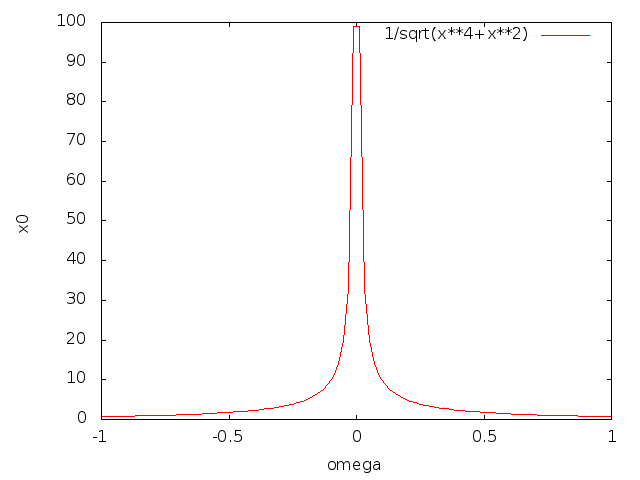
\includegraphics[width=10cm]{curve.png}
\end{center}
\end{figure}
\end{document}
